%!TEX root = haiku.tex
\book{\LARGE \FK 山头火俳句集}

\begin{figure}
    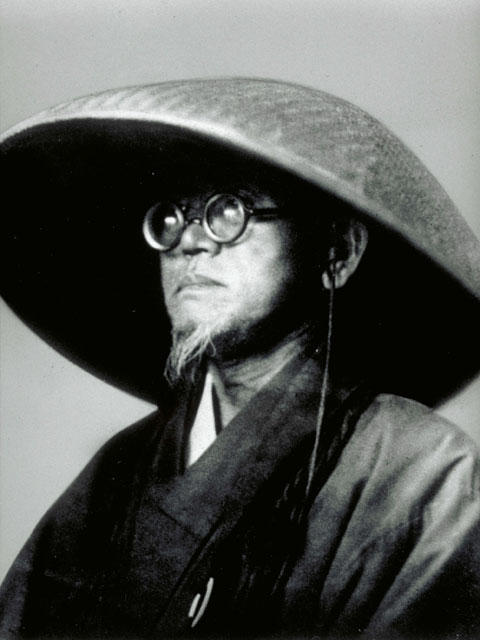
\includegraphics[width=\textwidth]{santoka}
\end{figure}

\chapter{\FK 献给祖父山头火}

{\FS

    \hfill 种田美奈子\footnotemark[1]

    \bigskip

    岁月流逝,在您逝世五十周年的时候,发生了一件难得而可喜的事情,这就是您的俳句被译成了中文。此刻我希望您的作品,能在同中国文化相结合的方面起到一定作用。

    回想起来,您走过了遥远的路程。一个人的足迹,竟然会同如此众多的人有着联系,您曾经这么问过自己吗?

    除了您走过的道路,没有能够找到维持生活的方法。您走过了自己认为无可奈何的道路。您得到了谅解您的人们的恩惠,才能够自始至终贯彻了创作自由律俳句\footnotemark[2]的意愿。这当然是您一生的憧憬。然而,您这样做,使我父亲陷入了孤独和苦恼的深渊\footnotemark[3]。说来,我已经到了时时感叹人生无常的年龄。我将凝眸等待您的作品的中文译本在中国出版,看它究意是什么样的面貌。最后,列出我所喜爱的您的俳句:

    \begin{quote}
        杜宇声声,明朝攀越彼山行。\\
        烈日炎炎,铁路笔直伸向前。
    \end{quote}

    \hfill 合掌

    \footnotetext[1]{\FS 本文作者是种田山头火的孙女,现住日本巧栖市。本文是她为日本版《山头火的世界·山头火秀句汉译集》撰写的前言。上梓前有所补充。本文为李芒译注。}
    \footnotetext[2]{\FS 传统俳句有五、七、五句式等格律,冲破格律,不拘音数句式等,即称自由律俳句。}
    \footnotetext[3]{\FS 山头火于一九二〇年、三十八岁时,与妻子协商离婚,由妻子扶养独生子健。尔后出家,继而开始托钵云游的生涯,并深入进句创作。因而,在生活上为亲友妻儿带来很多麻烦。}
}

\chapter{\FK 李芒先生为山头火增新辉}

{\FS

    \hfill 富永鸠山\footnotemark[1]

    \footnotetext[1]{\FS 本文作者是山头火研究会会长、著名书法家,本文是他为日本版《山头火的世界·山头火秀句汉译集》撰写的前言。本文为李芒译注。}

    \bigskip

    是俳句,还是痛苦\footnotemark[2],一开头,我就想这样写下去。山头火的生活道路和俳句创作,实际上都是在削割着自己的肉体,这也正是使得我非这样写下去不可的原因。

    \footnotetext[2]{\FS 俳句在日本也简称句(ku),ku和苦同音。}

    看上去,山头火象是在愚鲁中生活过来,也像随着罪孽的潮流漂泊不定。或者说,两者交错着,纠缠着,高迈和庸俗,美和丑,矜持和自嘲,安乐和悲哀,等等,只顾在思维和宿命的峡谷中,坚持不懈地摇橹行船。这样,山头火千真万确地生活了一个时代。他背负着一切,在创立一个世界,在自由律俳句创作方面,做出了历史上无与伦比的贡献。

    至今,关于山头火,发表过很多分析文章,应该说评价都是正确的。只是,我在同他唯一的儿子健先生一起旅行,询及山头火在味取观音堂的生活,然后又离开观音堂走上流浪行乞的旅途等经历,健先生只回答了一句话:「那是孤独的地狱。」这话在我听来最为鲜明,当时便反复想到到底是健先生直接同山头火接触过,话里充满真实的感情,而能打动听者的心弦。同时,也感觉到健先生自身的感情似乎是这样的。那么,在山头火心目中盘旋着的东西究竟是什么呢?也许连山头火本人也无法做出明确的回答,这只要看看山头火的生活、生平和俳句创作,也就会得到证明。

    山头火确实有着一种什么东西,能够使读者、研究者深思、沉醉和倾慕。观察一下他的句碑吧。山头火的句碑,当今在日本全国已建立了一百几十座。据说,要建的计划还很多,其中由个人建立的也达到相当的数目。这说明对山头火的倾慕达到了什么程度。

    铁钵会剧团上演的以山头火为主题的戏剧,把观众引进感动的热潮中去了。

    山头火的生平还被改编成电视剧和歌曲。真可以说,山头火已经使各个领域的人们感到了陶醉。

    一九八一年,山头火迎来了诞生一百周年纪念。当时,人们在收集资料的过程中,对山头火的评价分歧颇多。于是我想如若尽可能完整地把所有的山头火观收集起来,或许也是接近山头火的真实形象的一个手段。无论遭到怎样的歪曲,只要那形象活动在人们心目中,人们就会感受到一种真实,宝贵的真实,而这种真实又无疑是山头火所给与的影象。

    美国的乔·斯蒂文思先生出版了山头火的英译本,他通过对禅的研究发表了自己的研究论文和俳句的英译,为山头火文学增添了一个侧面,使人们看到更深一层的内含和扩展。

    我以书法为专业,是私塾的老师。因此,举行过三次日中友好书法展览。一九八五年,一个偶然的机会结识了当时在重庆市四川外语学院任教的宫本博子先生。她原是想把中国书法家介绍给我的。谈话中提到有位中国著名文学家正在研究山头火,收集资料,我就给这位先生寄去了一些。很快就收到回信,并附上墨书的山头火俳句和译文。汉字所固有的多样而深邃的表现力立刻就把我吸引住了。

    比如:
    \begin{quote}
        茕茕背影,缓步暮秋冷雨中。
    \end{quote}

    「茕茕」一词,辞典上说的是孤独无依,这种简洁而美妙的表现,赋与原作以生动的解释。

    这位译者就是中国社会科学院的李芒先生。我把自己受到的感动告诉了李芒先生,从此开始交往,曾经一度在东京做了彻夜长谈。山头火俳句集的中文译本在日本的出版,就这样迈开了第一步。

    这里,也出现了一位为山头火增新辉的人。

    于是,我们就是这样走近了山头火,山头火也展现出千姿百态。
    李芒先生不断地对译文进行推敲。他既注意到日中文化的差异,又苦心于确立自己的文学和山头火观。在中国,首次将日本的自由律俳句译成中文,这是一件需要决心和勇气的工作。

    中国,在翻译日本的定型俳句方面,已经在从事种种实验,还出现了「汉俳」这种形式,也就是说,用五、七、五句式把汉字排列在一起的形式。这种方法更接近俳句,正在得到普及。

    然而,现在是李芒先生向山头火的自由律俳句挑战,无疑这是具有历史意义的伟大挑战。看来,他的这种挑战已经在中国引起巨大的反响。大家知道,中国自古就有优秀的汉诗,它的形式已经在悠久的历史长河中固定下来。因此,如若没有相当的勇气和探索精神,是无法做到这一步的。我必须告诉读者,李芒先生倾注在山头火俳句翻译工作中的热情,是令人惊叹的!

    山头火俳句集日本版的出版,已经得到拥有版权的山头火家的慨允,也得到春阳堂出版社的支持。

    中国驻日大使馆一等秘书张光佩女士给以细致周到的指导和支持,也使我深受鼓舞,谨致衷心谢忱。

    另外,我最好的朋友肖宏先生始终同我合作,给予协助,亦借此机会致谢。

    山口县立图书馆的上野美代子女士、远藤制版绘图研究所的远藤夫妇、宇部高等学校的鹤田哲人先生以及防府彩色图片社的河合祥一先生等都给予大力支持,亦应致谢。

    这里,刊载了日本和中国书法家的作品,中国的有中国书法家协会理事费新我先生、北京篆刻家郑怀宝先生,日本的有书宗院院长、东宫书法进讲桑原翠邦先生等杰作,满足了我们和李芒先生的共同希望,使我们感到分外的光荣。

    最后,还要提出的是春阳堂书店和田欣之介社长、责任编辑永安浩美先生均曾给以无微不至的关怀。

    恰好在纪念山头火逝世五十周年的时候,我们遇到了这么多好人,得以使本书问世,确实是令人感激不尽的。

    在执笔撰写本文的过程中,有一种感想突然涌现在心头……

    这就是在这个不毛而又悖理的时代,要想跟山头火打交道,确实要怀有一颗求道而蕴含哲理的心。否则,是无法接近山头火的。

    这个山头火俳句的中文译本,如若能够加深日中两国的理解,有助于友好的文化交流,实为至幸。

    期待着李芒先生更加活跃。

    \bigskip

    \hfill 合掌
}

\chapter{\FK 喜读山头火佳句并赋汉俳六首}

{\FS \hfill 邹荻帆

    \begin{quote}
        岁暮读佳诗\\
        废寝忘餐人笑痴\\
        喜摘梅一枝

        细玩奇世珍\\
        一章一句一乾坤\\
        译作两传神

        斗笠落蜻蜓\\
        千秋独吟一俳人\\
        余晖青山青

        托钵寻诗行\\
        流水落花皆文章\\
        自有春芬芳

        蟋蟀曾伴眠\\
        俳人诗思能感天\\
        乡梦配管弦

        武士跛脚归\\
        曷若华章白鸽飞\\
        海外留心碑
    \end{quote}
}

\chapter{\FK 一个人的世界}

{\FS \hfill 李瑛

    种田山头火,这是一个陌生的日本诗人的名字,也正由于对这一陌生诗人的发现,使我们又得以认识了一个新的世界而感到兴奋和喜悦。

    世界,历史,人生和艺术,是多么真实而复杂的存在。属于它们的种种现象和生活在其中的人们的思想行为、甚或某些际遇,是美学家、哲学家研究探索的课题。

    山头火是这样一个人:他出生在日本大地主家庭,上过大学文学系,经过商,但辗转求业总不能持久,离婚后嗜酒参禅,曾因痛苦而自杀未遂,后被一和尚收留看守寺院,又因难以孤处,便一钵一笠漂泊乞讨。就这样,他走过了自己艰苦曲折的一生。在他所处的广阔背景下,他心灵深处的种种复杂思绪:欢乐,痛苦,感触和顿悟,凝成了数万首极富特色、独具个性的俳句,这是他人生阅历与体验的结晶,是他心灵自白的长卷。他在人生旅途的求索中,不断地发现着自己,寻找着自己,而我们则通过他的作品认识了一个人的世界。

    如今,他留下的这些俳句,同日本八世纪编成的古典诗歌总集二十卷的《万叶集》及其以后众多的日本和歌、俳句诗人所创作的卷帙浩繁的作品一样,巳成为日本人民诗歌宝库中重要的组成部分,受到人民的称誉,并越过大洋,在国外产生了很大影响。

    日本文学与中国文学有着源远流长的关系,特别是古典诗歌,尽管由于两国诗人所生活的地理、历史、政治、社会、思想、文化等多方面的原因,使之在思想倾向、人生态度和艺术见解等方面不尽一致,但却也有许多共同的方面,他们都在各自的限制中寻找充分袒露自己内心世界的自由。

    日本自《万叶集》问世以来,和歌在内容上,多为宫廷官吏和上层僧侣等应制与即兴咏怀之作,和人民现实生活距离较远,所咏对象也多是山川草木、自然景色,常常是触景生情,借以抒怀;虽然也有些表现个人贫困和民间习俗、民族风情的作品,但其接触领域和感情范围也不以广阔为尚;艺术上,则在传统规律的严格限制中,力求韵味含蓄、风格淡雅,由于篇幅短小,所以对语言文字的精练简约,要求很高。一般说来,从短歌派生出来的俳谐及其起句的独立形式俳句,除了将和歌这种崇尚高雅的艺术转到庶民手中,并增加了诙谐成分以外,基本上也是如此。而山头火的诗作,却打破了传统俳句定型格律的某些约束,追求自然淳朴,并强化语言的选择。他常常努力使作品负载更大的容量和产生高度的艺术表现力。通过自己的真挚感受,采取以小见大的手法,或隐喻,或暗示,使作品蕴含着深邃动人的感情。由于他不凡的经历,特别在他漂泊乞讨的生活中,行经各处,自然界的山山水水和各种物象,自然便成为他观察思考和表现的对象,他眼里的大自然也就全然不同于任何别人眼里的大自然。他通过自己饱尝人间酸甜苦辣和历经动荡之苦的观察感受,追求着一种意蕴和兴寄,借以抒发自己的情怀。

    在他一九二六年开始浪迹四方的乞讨生活之后几年,曾经历了十年侵略战争的年代,直到他一九四〇年去世。他既不从事物质生产,也不参加侵略战争,他既不笃信佛教的生死轮回,也不愿接近唯物的马克思主义;作为一个贫苦行僧,他只怀着满腔天真淳朴的感情,希望人与人不要互相残杀,而对人间疾苦、战乱死伤则表现了深挚的同情,任何人也不能不受历史的局限和制约。山头火就是这样一个人。译者李芒先生对他做了准确的研究和分析。是的,他就是这样一个人,一个具体存在的人,一个企望遁世却又不能与世隔绝的人,一个活生生的单纯而又复杂的人,他只相信「我在创造」,他是怀着一片诚挚的心「作我独自的真诚的诗」的。

    在他所经历的复杂感情与体验中,不少诗表现了他对勃勃生机的大自然的执着和由衷的爱。

    \begin{quote}
        几番晴日几番雨,稻苗青满畦。\\
        烟霞袅袅重重山,山是我家园。
    \end{quote}

    这里,通过稻田中满眼青青的禾苗和重峦间缭绕的烟霞,表现出作者何等强烈的对生活的赞美和眷恋情怀!有些还明显的融进了他睿智的哲学思考。

    在他放浪四方的空茫与孤寂中,在他低沉痛苦的行脚生涯中,自然会时时怀念离去的故里:

    \begin{quote}
        故乡归路遐,春树绽新芽。\\
        涛声只不断,故里巳遥远。\\
        皓月频招唤,故乡节庆酣。
    \end{quote}

    仿佛是一步一回首的深沉思念,联及此时此刻,此情此景,仔细玩味,字里行间渗透出浓重的难以名状的隐衷和复杂的感情。

    尽管他内心和境遇苦难重重,却始终未因困厄而绝望,他的不少诗虽难免染就孤凄悲凉的色调和一种虚幻的宗教感情,但更为深沉的是,从他的诗句中,传达出他对人世深层的慨叹和感喟,对人生忧患的某种彻悟,并且仍能从中发掘出美来。一只蜻蜓,一匹蟋蟀,远山近水,春花秋树,头上的云霞冷雨,脚下的碧草青禾,甚至屋檐融雪的滴水声,都蕴含着他无限真挚的思绪,成为一种美,一种宁静高洁的美、一种纯净的尊严美、一种能够撼动人们心灵的力量。

    说来奇怪,我在每每阅读日本短歌、俳句时,总觉得许多日本诗人都很善于运用绘画中的「留白」技法,使之以无胜有,以虚寓实。在作品中,虽然只作极少的细致的点染,而留出极富魅力的「艺术空白」,成为读者驰骋想象的天地,极大地丰富和补充了作品的意境和气氛,从而产生深长的韵味和强烈的艺术效果。

    \begin{quote}
        月色清明舟自横,且睡其中。
    \end{quote}

    这里山头火只写了月色皎洁,无以为家,在一只小舟中睡去,而读者读后得到的,除此之外,却兴起了更多的联想,诸如:一天长途跋涉行乞的劳顿,长空下月光照着寂寥的旷野、荒僻的河畔,也许是行经野渡,发现一只无人小舟,便进去睡了的野趣;在这里,读者不仅可以想象出作者此时的心境和神态,还仿佛可以看见河中的月光倒影,听见四野的虫鸣、水声,甚至可以闻见岸边潮湿里野艾蔓草的浓重气息……这种读者感觉中联想的景物的美,比起直观表达的景物的美,似乎更丰富,更强烈,更含蓄,因而也更耐人寻味。这种精心处理的「艺术空白」,大大拓展了人们的想象力,直接丰富了人们生命的容量,从而有助于人们的感情陶冶和心灵建设。

    作为一个特定时代的日本诗人的心灵经历,山头火对于我们确实是一片深沉广阔的大陆,一个奇异的世界。我想,中国读者对于他所袒露的自己不同寻常的真诚和单纯的心史,会是完全可以理解并热爱的。

    俳句在日本人民中间有广泛的群众基础,深受日本人民的喜爱。据说在日本,专业和业余的俳句作者至少有三百多万;他们有专门研究讨论俳句创作和活动的组织,有专门编辑出版俳句的刊物。俳句这种体制短小、极富民族特色的诗歌形式的创作,在日本正在得到日益繁荣和发展,在国外也正在产生越来越大的影响。

    李芒先生华生致力于日本文学研究和译著,是我国文学界十分熟悉的著名学者和翻译家。他不仅熟谙日本文学,而且对中国文学特别古典诗词也有很深的造诣。他译著颇丰,只就和歌和俳句的汉译问题,就曾写过多篇学术长文,引起国内和日本学者、专家的兴趣和重视。现在,又为我们介绍了一位早应结识的俳句诗人。俳句比起日本现代诗和短歌来,因其体制更短,语言的回旋余地更小,而各国文字又各有不同的规律和特点,所以翻译的难度更大,要求更高;李芒先生以其严肃认真的态度,力求最大限度地把原作的神韵和境界准确地表现出来,他对原作者的深刻研究和对译作的反复推敲,精益求精的严谨治学精神,是使人钦佩的。如今,他把鲜为我国读者所知的山头火的俳句在纪念诗人逝世五十周年的今天第一次介绍给我们,不仅有助于我们欣赏和借鉴他的诗作,进一步认识日本文学和日本诗歌的发展,也为增强中日两国文化交流、促进两国人民和诗人之间的友谊和了解作出了新的贡献,为此,我们应该衷心地感谢他。

    \bigskip

    \hfill 一九八九年二月十六日于北京
}

\chapter{\FK 山头火与自由律俳句}
{\FS

    \hfill 刘德有

    \bigskip

    在中国,把种田山头火这位日本俳人和他的俳句介绍给读者的,大概要算李芒同志是第一位了。我在《日语学习与研究》杂志(一九八六年第六期)上看到李芒同志发表的《论山头火并佳句选译》时,真有一种难以言状的喜悦。我佩服他的眼力,他的学识,他的胆量,更为他那一颗火一样的探求心所感动。

    李芒同志的论文,使我想起了一件事。那是一九八六年十一月,日本著名剧作家宫田三先生来北京,我们见面时他送我一本书,名叫《{\FM うしろ姿のしぐれていくか}》(茕然背影,缓步暮秋冷雨中\footnotemark[1])。翻开阅读,方知是一部剧本,写的是一位漂泊行乞的俳人种田山头火。「{\FM うしろ姿のしぐれていくか}」,既是剧名,也是这位俳人的代表作。

    \footnotetext[1]{\FS 本人引用的山头火俳句的译文,除注明者外,均出自李芒同志之手。}

    山头火这个名字,当时对于我是陌生的。不消说,他的俳句我也是第一次接触。读了山头火的俳句,使我感到新鲜、活泼、开阔、舒展,就像一个长年屈居斗室的人,突然看见了碧蓝的大海。

    俳句是日本韵文学的一种传统形式,也是世界上最短的格律诗。但,山头火向传统挑战,冲破格律,创作了上万首「自由律俳句」。他不受三节十七字(五、七、五)的束缚,他无视季题,也很少使用「切れ字」(断句的助词或助动词)。我们知道,在俳句史上,确有一些名家偶然也违背俳句禁律写一些灵动有致的句作。同时我们也知道,写「自由律俳句」也并非自山头火始。但应该说,山头火是向俳句传统进行挑战最为彻底的一个。

    诗,应该迸发生命的火花,发露诗人的情感。俳句也不例外。俳句要在被规定了音数的短句中表现诗人的世界。但是,仅仅音数齐整,做到了五、七、五,也未必就是俳句。例如「{\FM とびだすな車は急に止まれない}」,就不是俳句,而只是一条宣传交通规则的标语而巳。其次,即使合乎格律,音数齐整,含有季题,也未必就是一首好俳句。因为它虽然有外在的韵律美,但如果是「无病呻吟」,没有唱出作者的心声,就不是诗,因而就不能打动人。

    而山头火呢?他的俳句虽然不注重外在的韵律美,但它们着意奇拔,句句闪动着作者的灵感,句句具有神韵,句句是诗,因而不能不感人,不能不引起强烈共鸣。请看他的几首俳句。
    \begin{quote}
        {\FM 分け入つても分け入つても青い山}\\
        (拨草行行复行行,此身犹在青山中。)

        {\FM 朝の橋をわたるより乞いはじめる}\\
        (清晨过此桥,开始行乞讨。)

        {\FM 鉄鉢の中へも霰}\\
        (铁钵铮铮鸣,亦闻落霰声。)

        {\FM だまつて今日の草鞋穿く}\\
        (默默无言,且将今日草鞋穿。)

        {\FM こころわびしくひとりまた火を焚く}\\
        (胸怀寂然,独自又将炊火燃。)

        {\FM 笠にとんぼをとまらせてあるく}\\
        (且凭斗笠落蜻蜓,伴吾一路行。)

        {\FM 咳がやまない背中をたたく手がない}\\
        (连连咳嗽,却无为我捶背手。)

        {\FM 酔うてこほろぎと寝ていたよ}\\
        (陶然吃酒醉,蟋蟀曾同睡。)

        {\FM 寝ころべば枯草の春匂ふ}\\
        (躺一躺,但闻枯草散春芳。)
    \end{quote}

    山头火正是通过这些「自由律」俳句迸发出他的生命火花,表达了他的强烈情感。

    我这样说,丝毫也没有要贬低传统俳句的意思,相反地,我酷爱传统俳句。那些优美典雅,或风格清新,或情景交融,或触思抒怀的传统俳句,我认为只要它们是真正的诗,就具有艺术的魅力,就会感染读者,就能拨动人们的心弦。迄今为止,日本留下了那么多脍炙人口的传世名句,便是明证。然而,在山头火来说,他如果墨守格律,不采取自由律,也许是写不出那样生动活泼、清新泼辣的惊人之句的。山头火之所以要打破格律束缚,去追求自由律,我以为恐怕跟他的身世、经历、思想和艺术观有密不可分的关系。

    山头火(一八八二—一九四〇)是山口县防府市人,十一岁时母亲跳井自杀,使他精神上受到很大打击。他在早稻田大学文学系二年级就学时因患神经衰弱症中途退学返乡,跟父亲共同开办酿酒厂而宣告破产。后迁居熊本,三十九岁时与妻子离婚,并转赴东京谋生,但未获成功。他痛苦失望,生活放荡,进一步嗜酒,后返回熊本当了和尚,开始了「一钵千家饭」的行脚讨乞生涯。山头火生活的年代正是日本资本主义兴起发展,对外频频发动战争,国内各种矛盾日益激化的年代。这些都决定了他复杂的世界观:他叹息人生无常,感到寂寥、孤寒,但他热爱生活,热爱大自然;他是一个不折不扣的人道主义者,他不希望人与人互相残杀,但无法洞察战争的本质。激烈动荡的社会,无情地拨弄着他的命运,但他一心希望能成为一个诚实的人,努力进行他的俳句创作。山头火写道:「天不灭我,叫我作诗;我活着作诗,作我独自的真诚的诗。」我们可以说,恰恰是山头火的生活内容,决定了他采用自由律的形式写俳句;而自由律俳句又最好地最生动地表现了他的生活、他的思想和情感。

    也许有人会说,「写自由律俳句,不是无异于写短句的自由诗吗?」「格律和季语是俳句的生命,否定了它们,不就是否定俳句本身吗?」「既要写俳句,又要打破格律,山头火不是自相矛盾吗?」是的,山头火选择的,正是一条矛盾的路。诚然,他冲破了俳句的格律,但他没有放弃俳句。他在坚持俳句的过程中,去反抗被视为俳句生命的各种格律的束缚,给俳句注入了新的生命。艺术从来贵在创新,艺术要求个性。从这个意义上说,山头火的俳句打破格律,完全符合艺术的规律,它本身就是艺术,或者说它反映了山头火的艺术观。

    我们知道,传统俳句有季语,是日本风土培育出来的日本人的美意识的反映,它同日本美丽的大自然和四季的更换以及生活在这一自然环境中的日本人的异常细腻而反应十分灵敏的情感、心态等有着密不可分的关系。山头火同样也生活在这样的大自然和环境之中。他虽然不受季语的束缚,但也不是绝对不使用季语。上述「{\FM うしろ姿のしぐれていくか}」「{\FM 鉄鉢の中へも霰}」句中的「{\FM しぐれ}」、「{\FM 霰}」就是季语。但山头火不是把它们作为季语,而是作为映入他眼中的自然景物写进了俳句之中。这就是说,山头火尽管反对格律,不受季语束缚,不去有意识地歌唱季节,但他也终于不能摆脱季节,不能脱离开俳句本身。

    按习惯,日本的短歌和俳句常常在句前加题,或附以小序,以便有助于读者加深对这些短歌或俳句的理解,而不使人们感到唐突。但山头火的俳句却极少加题或附以小序。即使这样,也不使人感到唐突而能够很好地理解它,这是因为读他的俳句的人一般都了解他的生活经历的缘故。从某种意义上说,山头火的生活和他的云游本身就是他的俳句的序。而这同时也是他的自由律得以成立的最大因素。山头火的自由律俳句,乍一看似乎是随便写写,不经推敲,写完了事。但实际上,他无论走到哪里,总是带着笔记本和一支钢笔,不知疲倦地写,不断地修改,不断地推敲。由此可见,他的创作态度是严肃的。

    \begin{quote}
        {\FM 雨ふるふるさとははだしであるく}\\
        (故乡冷雨中,托钵归来赤脚行。)
    \end{quote}

    读了这首俳句,无需多加说明,在我们眼前浮现的是这样一幅景象:头戴斗笠,手持铁钵,身披黑袍的山头火来到山口县旧居门前。如今他巳成为行乞的僧人,他不愿被熟人认出他来,便故意把斗笠戴得很深,在雨中赤脚匆匆走过。

    还有,据说山头火在旅行时腰间总是缠着一个包裹,里面包的是自杀了的母亲的牌位。他一生中写了许多怀念母亲的俳句,可见他对母亲有着深厚的感情。他在母亲忌日那一天,创作了这样的俳句:

    \begin{quote}
        {\FM うどん供えて、母よ、わたくしもいただきまする}\\
        (面条供灵前,母亲哟,儿与您老同吃面。\footnotemark[1])
    \end{quote}

    \footnotetext[1]{\FS 此句为笔者所译。}

    山头火的诗句虽没有气魄宏大、苍茫深沉的风格,但有寄托感慨、意境深远的铺述手法。他的俳句,语言简明平易,但表现出深邃的内涵,具有艺术的魅力和美学价值。

    山头火在运用语言和造句方面,确实是独具匠心的。在日语中,五音和七音的句子读起来,琅琅上口,节奏感很强。这是「五、七、五、七、七」的短歌和「五、七、五」的俳句得以广泛流传的重要条件。为什么山头火的那些打破这一格律的自由律俳句也能使人读起来感到优美和谐、铿锵有力呢?我想,这是因为山头火虽然写的是不规则句子,但仍注意节奏感的缘故,例如「{\FM うしろ姿のしぐれていくか}」(音数为两节,七、七音),「{\FM 月がまねくふるさとはおまつり}」(三节,六、五、四),「{\FM 炎天をいただいて乞い歩く}」(三节,五、五、五),「{\FM 水のうまさを蛙鳴く}」(二节,七、五),「{\FM わがままきままな旅の雨にぬれてゆく}」(三节,八、六、五),「{\FM 落葉しつくしたる木の実の赤く}」(二节,九、六)。从以上的分析来看,这些句子中有许多五音和七音。这一现象是饶有兴趣的。这也表明山头火自由律俳句的语言,通过运用节奏感很强的五、七音加强了艺术效果。

    俳句,从它的发生和发展来看,走过了不断革新的道路。我们完全有理由说,随着时代的变迁,那种严守格律的传统俳句,今后也将在不断创新中继续发展。而自由律俳句,作为俳句发展中的一个流派,自有它产生的客观条件。自由律俳句的兴起,使传统俳句也吸收了有生命力的因素。而山身火对传统的反抗和挑战,实际上在客观上也起了使传统俳句以某种形式得到加强的作用。这大概就是事物的辨证法吧。

    山头火,是他的家乡山口县防府市的骄傲。

    最近,听说山口县防府市要把李芒同志的论文连同他翻译的山头火的俳句汇编成册,付梓出版,这是令人十分高兴的事。我对此表示衷心祝贺。我认为该书的出版一定能在中日两国人民、两国文学家的心灵与心灵中间架起一座友谊和相互了解的桥梁。

    李芒同志是我的挚友,我与他最早相识,是一九六一年春在东京举行亚非作家紧急会议时。那时我们作为代表团的成员第一次合作,他给我留下了深刻的印象。李芒同志为人诚挚、谦和、热情、朴实,具有长者风度。他知识渊博,特别是对日本文学有很深的造诣。当我知道他在中专读了一年书后便参加工作,年轻时做过火车司炉,而他的渊博的学识和高水平的日语是后来全靠自学掌握的时候,更加钦佩和尊敬他。

    李芒同志曾翻译过许多日本小说,也写过不少关于日本文学的评介。最近几年,他花费大量的精力和时间翻译介绍和歌、俳句。他在和歌与俳句的翻译实践方面有很多大胆的尝试和创新,丰富了我国翻译日本韵文的实践。不仅如此,更加可贵的是,李芒同志把他在翻译和歌俳句方面获得的经验上升为理论,提出了一些重要的独到的见解。我们知道,韵文的翻译是极为困难的。翻译和歌、俳句也是如此。李芒同志主张译者要「深入体会原诗的思想感情和艺术特点,与诗人打成一片」。他认为,原作与译文「都是『创作』,但却是两种不同的创作」。译者在把诗人的艺术品译成另外一种文字时,要「在力争将原作的内容与形式最大限度忠实地翻译出来方面进行创作,并努力使译文成为基本上与原作相同的艺术品。」他认为,「短歌和俳句内容各异,形式不一,从而译文也应主要从内容出发,注重神韵、风格和节奏的表现,兼顾形式的其他方面。」「总的精神是在釆取灵活多样的形式和方法的基础上,逐步增多地釆取适当的定型化的译法。」他主张,在「语言方面,一方面采取古典诗歌的格调,尽可能照顾到平仄规律」,「实在译不成者也在适当照顾到平仄规律的前提下译成古诗、长短句等。一方面既釆取古典诗歌的形式,又照顾到便于今人阅读,适当采用较之原歌原句稍微平易的词语,避免过分古雅难懂。」我认为,这些意见都是颇值得倾听的。李芒同志这次翻译山头火的自由律俳句,就采取了古诗的格律,尽量使用平易语言,即口语古调的方法。正是李芒同志基于这一原则的辛勤劳动,今天使更多的中国读者和日本文学爱好者读到了山头火的作品。

    当然,翻译和歌、俳句,完全可以有各种不同的方法。有关日本传统韵文的翻译理论研究尚待进一步深化,同时理论创造也允许有不同的见解和主张。我们在科学和学术领域里实行「百家争鸣」,无疑有利于促进我国的科学学术事业的不断发展。我期望在和歌、俳句的汉译方面能出现一个互相展开意译、「百花齐放」,「百家争鸣」的繁荣局面。

    李芒同志作为日本文学研究会副会长、中国外国文学学会常任理事、中国翻译工作者协会理事,为译介日本文学作品已经作出了很大贡献。希望他今后继续奋起健笔,在这一方面取得更丰硕的成果。我想,这绝不只是我一个人的愿望吧。

    作为一个日本文学爱好者的后辈,我不揣冒昧写了这一些不成熟的想法,是为序。
}

\chapter{\FK 本文}
\setcounter{haikucounter}{0}

\begin{haiku}
    {\FH 松風に明け暮れの鐘\ruby[g]{撞}{つ}いて。}

    {\FK 飒飒松风,撞罢晨钟又暮钟。}
\end{haiku}

\begin{haiku}
    {\FH ひさしぶりに掃く\ruby[g]{垣根}{かきね}の花が咲いてゐる。}

    {\FK 久疏持帚来,欲扫篱笆花正开。}
\end{haiku}

\begin{haiku}
    {\FH 分け入つても分け入つても青い山。}

    {\FK 拨草行行复行行,此身犹在青山中。}

    {\FS 此句前言为「大正十五年(一九二六)四月,背负着无法解决的迷惑、走上行乞流浪的旅途」,表现了找不到出路的情绪。}
\end{haiku}

\begin{haiku}
    {\FH しとどに濡れてこれは道しるべの石。}

    {\FK 雨淋精湿,却是一枚指路石。}
\end{haiku}

\begin{haiku}
    {\FH 炎天をいただいて\ruby[g]{乞}{こ}ひ歩く。}

    {\FK 头顶烈炎天,化缘走向前。}
\end{haiku}

\begin{haiku}
    {\FH 鴉啼いてわたしも一人。}

    {\FK 孤鸦一声鸣,吾亦一人行。}
\end{haiku}

\begin{haiku}
    {\FH 生死の中の雪ふりしきる。}

    {\FK 生死轮回中,霏霏白雪积重重。}

    {\FS 此句前言为「认清生死乃佛家一大事之因缘也」。}
\end{haiku}

\begin{haiku}
    {\FH 木の葉散る歩きつめる。}

    {\FK 树叶正飘零,云游步不停。}
\end{haiku}

\begin{haiku}
    {\FH 張りかへた\ruby[g]{障子}{しょうじ}のなかの一人。}

    {\FK 格子拉门新糊过,室中只我一人坐。}
\end{haiku}

\begin{haiku}
    {\FH 踏みわける萩よすすきよ。}

    {\FK 芒草胡枝子,拨开踏倒步迟迟。}

    {\FS 此句前言为「昭和二、三年(一九二七、八),毫无目标地徘徊在山阳道、山阴道和四国九州一带」。}
\end{haiku}

\begin{haiku}
    {\FH この旅、果もない旅のつくつくぼうし。}

    {\FK 此次云游,寒蝉孤飞无尽头。}
\end{haiku}

\begin{haiku}
    {\FH へうへうとして水を\ruby[g]{味}{あじわ}ふ。}

    {\FK 悠然独享,且将清水味道尝。}
\end{haiku}

\begin{haiku}
    {\FH 落ちかかる月を観てゐるに一人。}

    {\FK 月亮正西沉,遥望只一人。}
\end{haiku}

\begin{haiku}
    {\FH \ruby[g]{投}{な}げだしてまだ陽のある脚。}

    {\FK 坐地伸双腿,脚上悠然尚落晖。}
\end{haiku}

\begin{haiku}
    {\FH 山の奥から繭負うて来た。}

    {\FK 人自深山外,遥遥负茧来。}
\end{haiku}

\begin{haiku}
    {\FH 笠にとんぼをとまらせてあるく。}

    {\FK 且凭斗笠落蜻蜓,伴吾一路行。}
\end{haiku}

\begin{haiku}
    {\FH 歩きつづける彼岸花咲きつづける。}

    {\FK 行走不停步,曼珠沙华开一路。}

    {\FS「曼珠沙华」据说原意为红色,日本称彼岸花、天涯花、死人花、幽灵花、舍子花等。曼珠沙华是日本的梵文译音。它有毒而多生于墓地,一般认为是不吉利的花,然而秋季一枝能开多朵嫣红的花,很美。中国称石蒜、龙爪花、蟑螂花等。}
\end{haiku}

\begin{haiku}
    {\FH まつすぐな道でさみしい。}

    {\FK 只有笔直路一条,行来更寂寥。}
\end{haiku}

\begin{haiku}
    {\FH だまつて今日の草鞋\ruby[g]{穿}{は}く。}

    {\FK 默默无言,且将今日草鞋穿。}
\end{haiku}

\begin{haiku}
    {\FH ほろほろ酔うて木の葉ふる。}

    {\FK 树叶落翩翩,犹如酒醉飘飘然。}
\end{haiku}

\begin{haiku}
    {\FH しぐるるや死なないでゐる。}

    {\FK 冬初雨凄凄,人犹未死去。}
\end{haiku}

\begin{haiku}
    {\FH 水に影ある旅人である。}

    {\FK 水中投影有吾身,吾本一旅人。}
\end{haiku}

\begin{haiku}
    {\FH しぐるるやしぐるる山へ歩み入る。}

    {\FK 冬初雨凄凄,雨中走进深山去。}
\end{haiku}

\begin{haiku}
    {\FH 生き残つたからだ\ruby[g]{掻}{か}いてゐる。}

    {\FK 此身得以活下来,搔痒怡心怀。}
\end{haiku}

\begin{haiku}
    {\FH また見ることもない山が遠ざかる。}

    {\FK 相识无缘又一山,离吾渐渐远。}
\end{haiku}

\begin{haiku}
    {\FH どうしようもないわたしが歩いてゐる。}

    {\FK 心怀无可奈何情,独自向前行。}
\end{haiku}

\begin{haiku}
    {\FH 分け入れば水音。}

    {\FK 拨草走进深山中,且闻流水声。}
\end{haiku}

\begin{haiku}
    {\FH すべつてころんで山がひつそり。}

    {\FK 滑倒又跌倒,山岭静悄悄。}
\end{haiku}

\begin{haiku}
    {\FH すつかり枯れて豆となつてゐる。}

    {\FK 枝叶尽干枯,却有豆成熟。}
\end{haiku}

\begin{haiku}
    {\FH 捨てきれない荷物のおもさまへうしろ。}

    {\FK 家什不肯丢,沉重背前后。}
\end{haiku}

\begin{haiku}
    {\FH あの雲がおとした雨にぬれてゐる。}

    {\FK 我身淋湿雨纷纷,降自中天那片云。}
\end{haiku}

\begin{haiku}
    {\FH 年とれば故郷こひしいつくつくぼうし。}

    {\FK 人到老年,萦怀故里一秋蝉。}
\end{haiku}

\begin{haiku}
    {\FH 水音といつしよに里へ下りて来た。}

    {\FK 水声作伴,下山来到小村前。}
\end{haiku}

\begin{haiku}
    {\FH まつたく雲がない笠をぬぎ。}

    {\FK 长空闲静无云翼,摘下斗笠。}
\end{haiku}

\begin{haiku}
    {\FH 墓がならんでそこまで波がおしよせて。}

    {\FK 坟墓并排一座座,涌向前来有海波。}
\end{haiku}

\begin{haiku}
    {\FH 酔うてこほろぎと寝てゐたよ。}

    {\FK 陶然吃酒醉,蟋蟀曾同睡。}
\end{haiku}

\begin{haiku}
    {\FH 雨だれの音も年とつた。}

    {\FK 茅檐滴雨声,竟亦临衰境。}
\end{haiku}

\begin{haiku}
    {\FH 物乞ふ家もなくなり山には雲。}

    {\FK 再乞食巳无人家,且眺望山上云霞。}
\end{haiku}

\begin{haiku}
    {\FH 笠も\ruby[g]{漏}{も}りだしたか。}

    {\FK 侬一斗笠,亦漏潇潇雨。}
\end{haiku}

\begin{haiku}
    {\FH 霜夜の\ruby[g]{寝床}{ねどこ}がどこかにあらう。}

    {\FK 霜夜沉沉,总有一处可安身。}
\end{haiku}

\begin{haiku}
    {\FH うしろすがたのしぐれてゆくか。}

    {\FK 茕然背影,缓步暮秋冷雨中。}

    {\FS 此句标题为「自嘲」,并有前言说:昭和六年(一九三一),本想在熊本市落脚,但终未成功,只好继续云游四方,别无良策。}
\end{haiku}

\begin{haiku}
    {\FH \ruby[g]{鉄鉢}{てつぱつ}の中へも霰。}

    {\FK 铁钵铮铮鸣,亦闻落霰声。}
\end{haiku}

\begin{haiku}
    {\FH ふるさとは遠くして木の芽。}

    {\FK 故乡归路遐,春树绽新芽。}
\end{haiku}

\begin{haiku}
    {\FH 笠へぽつとり椿だつた。}

    {\FK 忽闻斗笠响一声,却是山茶正落英。}
\end{haiku}

\begin{haiku}
    {\FH 今日の道のたんぽぽ咲いた。}

    {\FK 今日行小径,着花喜见蒲公英。}
\end{haiku}

\begin{haiku}
    {\FH 雨ふるふるさとははだしであるく。}

    {\FK 故乡冷雨中,托钵归来赤脚行。}
\end{haiku}

\begin{haiku}
    {\FH うつりきてお彼岸花の花ざかり。}

    {\FK 方始迁来,曼珠沙华正盛开。}
\end{haiku}

\begin{haiku}
    {\FH 草の\ruby[g]{実}{さね}の露のおちつかうとする。}

    {\FK 草籽宿露珠,似欲且长住。}
\end{haiku}

\begin{haiku}
    {\FH ゆふ空から柚子の一つをもらふ。}

    {\FK 遥对晚霞如锦绣,且来索取一颗柚。}
\end{haiku}

\begin{haiku}
    {\FH 月が昇つて何を待つでもなく。}

    {\FK 皓月东升入碧穹,并非怀有待何情。}
\end{haiku}

\begin{haiku}
    {\FH ひとりの火の燃えさかりゆくを。}

    {\FK 独将炊火燃,愈旺愈开颜。}
\end{haiku}

\begin{haiku}
    {\FH 誰か来さうな空が曇つてゐる枇杷の花。}

    {\FK 似有谁人来我家,阴天喜绽枇杷花。}
\end{haiku}

\begin{haiku}
    {\FH 音は朝から木の実をたべに来た鳥か。}

    {\FK 何物枝头闹?必是啄食树籽声,小鸟飞来早。}
\end{haiku}

\begin{haiku}
    {\FH ぬいてもぬいても草の\ruby[g]{執着}{しゅうじゃく}をぬく。}

    {\FK 拔来又拔去,拔不尽青草执着意。}
\end{haiku}

\begin{haiku}
    {\FH もう明けさうな窓あけて青葉。}

    {\FK 似近黎明,推窗唯见叶青青。}
\end{haiku}

\begin{haiku}
    {\FH すつばだかへとんぼとまらうとするか。}

    {\FK 试问蜻蜓,欲在赤光身上停?}
\end{haiku}

\begin{haiku}
    {\FH かさりこそり音させて鳴かぬ虫が来た。}

    {\FK 窸窸窣窣发轻声,虫豸爬来却不鸣。}
\end{haiku}

\begin{haiku}
    {\FH 花いばら、ここの土とならうよ。}

    {\FK 野薇开簇簇,吾身欲作此处土。}
\end{haiku}

\begin{haiku}
    {\FH 山のいちにち蟻もあるいてゐる。}

    {\FK 一日山中方独步,却知蚂蚁犹行路。}
\end{haiku}

\begin{haiku}
    {\FH 雲がいそいでよい月にする。}

    {\FK 只为月亮更清丽,白云迅飞去。}
\end{haiku}

\begin{haiku}
    {\FH けふはおわかれの\ruby[g]{糸瓜}{へちま}がぶらり。}

    {\FK 今日将分手,丝瓜亦垂头。}
\end{haiku}

\begin{haiku}
    {\FH かすんでかさなつて山がふるさと。}

    {\FK 烟霞缥渺重重山,山是我家园。}
\end{haiku}

\begin{haiku}
    {\FH 春風の鉢の子一つ。}

    {\FK 春风和煦,铁钵伴我云游去。}
\end{haiku}

\begin{haiku}
    {\FH ひさびさもどれば\ruby[g]{筍}{たかんな}によきによき。}

    {\FK 久别归庵望,竹笋正呈祥。}
\end{haiku}

\begin{haiku}
    {\FH 家を持たない秋がふかうなるばかり。}

    {\FK 无家可归宿,唯有清秋暮。}
\end{haiku}

\begin{haiku}
    {\FH わがままきままな旅の雨にはぬれてゆく。}

    {\FK 咨情行旅处,一路雨淋湿漉漉。}
\end{haiku}

\begin{haiku}
    {\FH びつしょり濡れて代掻く馬は叱られてばかり。}

    {\FK 耙田耕马尽淋湿,却总受呵叱。}
\end{haiku}

\begin{haiku}
    {\FH はれたりふつたり青田になつた。}

    {\FK 几番晴日几番雨,稻苗青满畦。}
\end{haiku}

\begin{haiku}
    {\FH 草しげるそこは死人を焼くところ。}

    {\FK 碧草萋萋,此处原为火葬地。}
\end{haiku}

\begin{haiku}
    {\FH 炎天かくすところなく水のながれくる。}

    {\FK 炎天无处藏身影,清流却送水泠泠。}
\end{haiku}

\begin{haiku}
    {\FH 日ざかりのお地蔵さまの顔がにこにこ。}

    {\FK 阳光照耀,地藏菩萨面含笑。}
\end{haiku}

\begin{haiku}
    {\FH 待つでも待たぬでもない雑草の月あかり。}

    {\FK 似等非等自多情,杂草莹莹皓月明。}
\end{haiku}

\begin{haiku}
    {\FH 蚊帳へまともな月かげも誰か来さうな。}

    {\FK 蚊帐清明笼月影,似有谁来慰孤零。}
\end{haiku}

\begin{haiku}
    {\FH 散るは柿の葉咲くは茶の花ざかり。}

    {\FK 柿叶方凋残,茶花正竞妍。}
\end{haiku}

\begin{haiku}
    {\FH 空のふかさは落葉しづんでゐる水。}

    {\FK 欲度天空深几许,且观落叶沉水底。}
\end{haiku}

\begin{haiku}
    {\FH うしろから月のかげする水をわたる。}

    {\FK 月光来背后,踏影渡河流。}
\end{haiku}

\begin{haiku}
    {\FH とぼしいくらしの屋根の雪とけてしたたる。}

    {\FK 家贫屋顶雪莹莹,春日且闻滴水声。}
\end{haiku}

\begin{haiku}
    {\FH 焚くだけの枯木はひろへた山が晴れてゐる。}

    {\FK 拾得干柴足烧饭,晴光一片照山峦。}
\end{haiku}

\begin{haiku}
    {\FH よびかけられてふりかへつたが落葉林。}

    {\FK 忽闻呼唤方回首,却是林中落叶稠。}
\end{haiku}

\begin{haiku}
    {\FH 雪のあかるさが家いつぱいのしづけさ。}

    {\FK 瑞雪莹莹,室内清光一片静。}
\end{haiku}

\begin{haiku}
    {\FH ふくろうはふくろうでわたしはわたしでねむれない。}

    {\FK 我自幽居枭自鸣,长夜梦难成。}
\end{haiku}

\begin{haiku}
    {\FH けさは水音も、よいたよりでもありさうな。}

    {\FK 今朝水声亦含情,似有佳音慰茕茕。}
\end{haiku}

\begin{haiku}
    {\FH 生えて伸びて咲いてゐる幸福。}

    {\FK 发芽生长又开花,幸福应无涯。}
\end{haiku}

\begin{haiku}
    {\FH 閉めて一人の障子を虫が来てたたく。}

    {\FK 一人独处闭拉门,却闻虫豸叩频频。}
\end{haiku}

\begin{haiku}
    {\FH 山から山がのぞいて梅雨晴れ。}

    {\FK 此山望彼山,梅雨方停晴满天。}
\end{haiku}

\begin{haiku}
    {\FH 食べる物はあつて酔ふ物もあつて雑草の雨。}

    {\FK 有物可食有酒醉,杂草雨霏霏。}
\end{haiku}

\begin{haiku}
    {\FH いつでも死ねる草が咲いたり実つたり。}

    {\FK 草花开放又结实,观此随时均可死。}
\end{haiku}

\begin{haiku}
    {\FH 日ざかり落ちる葉のいちまい。}

    {\FK 烈日炎炎,落叶孑然只一片。}
\end{haiku}

\begin{haiku}
    {\FH ふるさとの水をのみ水をあび。}

    {\FK 故里水粼粼,润喉又洗身。}
\end{haiku}

\begin{haiku}
    {\FH お彼岸のお彼岸花をみほとけに。}

    {\FK 曼珠沙华春分摘,献与佛爷免祸灾。}
\end{haiku}

\begin{haiku}
    {\FH 彼岸花さくふるさとはお墓のあるばかり。}

    {\FK 曼珠沙华开簇簇,故乡处处皆坟墓。}
\end{haiku}

\begin{haiku}
    {\FH 重荷を負うてめくらである。}

    {\FK 背负重荷行,双目已失明。}
\end{haiku}

\begin{haiku}
    {\FH 月も水底に旅空がある。}

    {\FK 羁旅青空沉水底,且看皓月为佳侣。}
\end{haiku}

\begin{haiku}
    {\FH 昼寝さめてどちらを見ても山。}

    {\FK 午睡方睁眼,望去周遭尽是山。}
\end{haiku}

\begin{haiku}
    {\FH よい宿でどちらも山で前は酒屋で。}

    {\FK 好旅宿,四面青山对门是酒铺。}
\end{haiku}

\begin{haiku}
    {\FH ここで寝るとする草の実のこぼれる。}

    {\FK 草籽频频飞,便于此处睡。}
\end{haiku}

\begin{haiku}
    {\FH うらに木が四五本あればつくつくぼうし。}

    {\FK 房后有树四五株,必有秋蝉鸣不住。}
\end{haiku}

\begin{haiku}
    {\FH よい道がよい建物へ、焼場です。}

    {\FK 好路直通上好房,却是火葬场。}
\end{haiku}

\begin{haiku}
    {\FH 春が来た水音の行けるところまで。}

    {\FK 春风来顾,要赴水声流到处。}
\end{haiku}

\begin{haiku}
    {\FH この道しかない春の雪ふる。}

    {\FK 只此一条路,霏霏春雪轻移步。}
\end{haiku}

\begin{haiku}
    {\FH いつとなくさくらが咲いて逢うてはわかれる。}

    {\FK 春樱不觉绽繁英,相逢又叙惜别情。}
\end{haiku}

\begin{haiku}
    {\FH 燕とびかふ旅から旅へ草鞋を穿く。}

    {\FK 燕子频飞旋,云游此处又彼处,均把草鞋穿。}
\end{haiku}

\begin{haiku}
    {\FH 山ふかく\ruby[g]{蕗}{ふき}のとうなら咲いてゐる。}

    {\FK 山深若问有何花,总有款冬慰咱家。}
\end{haiku}

\begin{haiku}
    {\FH 日かげいつか月かげとなり木のかげ。}

    {\FK 日影何时成月影,皆为树影。}
\end{haiku}

\begin{haiku}
    {\FH 誰も来ないとうがらし赤うなる。}

    {\FK 无人来访,辣椒径自放红光。}
\end{haiku}

\begin{haiku}
    {\FH 枯れゆく草のうつくしさにすわる。}

    {\FK 草渐枯黄方显美,召吾坐下歇歇腿。}
\end{haiku}

\begin{haiku}
    {\FH 霽れて元日の水がたたへていつぱい。}

    {\FK 光风霁日迎元旦,桶中存水清又满。}
\end{haiku}

\begin{haiku}
    {\FH しぐれつつうつくしい草が身のまはり。}

    {\FK 遍体淋湿雨潇潇,周遭翠美深秋草。}
\end{haiku}

\begin{haiku}
    {\FH 人声のちかづいてくる木の芽あかるく。}

    {\FK 人声走近来,树芽放异彩。}
\end{haiku}

\begin{haiku}
    {\FH 草のそよげば何となく人を待つ。}

    {\FK 野草频摇摆,自是待人来。}
\end{haiku}

\begin{haiku}
    {\FH 何を求める風の中ゆく。}

    {\FK 此身何所求,迎风向前走。}
\end{haiku}

\begin{haiku}
    {\FH 草を咲かせてそしててふちよをあそばせて。}

    {\FK 着草开繁花,着蝶来玩耍。}
\end{haiku}

\begin{haiku}
    {\FH 青葉の奥へなほ径があつて墓。}

    {\FK 绿叶幽深犹有路,通向坟墓。}
\end{haiku}

\begin{haiku}
    {\FH 木かげは風がある旅人どうし。}

    {\FK 树荫吹清风,旅人喜共同。}
\end{haiku}

\begin{haiku}
    {\FH 月のあかるさがうらもおもてもきりぎりす。}

    {\FK 月光莹莹,庵前庵后蟋蟀声。}
\end{haiku}

\begin{haiku}
    {\FH あんたが来てくれさうなころの風鈴。}

    {\FK 君似将来临,风铃已报信。}

    {\FS 此句前言为「给树明君」。树明是作者朋友。}
\end{haiku}

\begin{haiku}
    {\FH こころむなしくあらなみのよせてはかへし。}

    {\FK 心境空空,激浪扑来又回腾。}
\end{haiku}

\begin{haiku}
    {\FH 水音とほくちかくおのれをあゆます。}

    {\FK 水声远处又近处,召我不停步。}
\end{haiku}

\begin{haiku}
    {\FH てふてふひらひらいらかをこえた。}

    {\FK 孤蝶翩翩,飞过屋甍舞碧天。}
\end{haiku}

\begin{haiku}
    {\FH 今日の足音のいちはやく橋をわたりくる。}

    {\FK 今日足音何其早,行人已渡桥。}
\end{haiku}

\begin{haiku}
    {\FH からむものがない\ruby[g]{蔓草}{つるくさ}の枯れてゐる。}

    {\FK 无物可缠绕,野径枯蔓草。}
\end{haiku}

\begin{haiku}
    {\FH 立ちどまると水音のする方へ道。}

    {\FK 行行又站定,水声来处有蹊径。}
\end{haiku}

\begin{haiku}
    {\FH 冬木の月あかり寝るとする。}

    {\FK 明月透光冬树间,就此且安眠。}
\end{haiku}

\begin{haiku}
    {\FH やつぱり一人はさみしい枯草。}

    {\FK 独自一人仍寂寥,默然对枯草。}
\end{haiku}

\begin{haiku}
    {\FH 落葉してさらにしたしくおとなりの灯の。}

    {\FK 落叶纷纷,邻家灯火倍相亲。}
\end{haiku}

\begin{haiku}
    {\FH ぼろ着て着ぶくれておめでたい顔で。}

    {\FK 褴褛一身臃肿相,唯有面孔喜洋洋。}
\end{haiku}

\begin{haiku}
    {\FH みぞるる朝のよう燃える木に木をかさね。}

    {\FK 清晨堆木一重重,雨雪交加火更浓。}
\end{haiku}

\begin{haiku}
    {\FH しみじみ生かされてゐることがほころび\ruby[g]{縫}{ぬ}ふとき。}

    {\FK 破衣缝补一针针,得以生存感慨深。}
\end{haiku}

\begin{haiku}
    {\FH 日ざかりの千人針の一針づつ。}

    {\FK 烈日炎炎一片心,街上千人各一针。}

    {\FS 以下十二句,附有总标题「后方」,写于一九三七年日军发动全面侵华战争以后。在这一组句作前面,有这样的序诗:「天不灭我,令我作诗。我活在世上,就要作诗,作我自己真诚的诗。」此句标题为「街头所见」,是客观的写生。「千人针」是日本妇女为保佑日军「武运长久」和亲人平安归来,请街头过路妇女用红线在白布上毎人缝一个结。据信达到千人千结后,便有效应。}
\end{haiku}

\begin{haiku}
    {\FH 月のあかるさはどこを爆撃してゐることか。}

    {\FK 月光朗朗,不知又在炸何方?}
\end{haiku}

\begin{haiku}
    {\FH しぐれて雲のちぎれゆく支那をおもふ。}

    {\FK 冷雨凄凄,思中国,云碎西飘去。}

    {\FS 原文中「支那」一词,据称是「秦」的梵文译音的汉字写法,日本从江户时代(一六〇三—一八六七)中期已通用。后来,逐渐有了蔑称我国的含义,第二次大战后,不再使用。山头火这里只是一般袭用。「云碎西飘去」一句,可能是暗示日军的覆灭。}
\end{haiku}

\begin{haiku}
    {\FH ひつそりとして八つ手花咲く。}

    {\FK 未闻人语,八角金盘花寂寂。}

    {\FS 此句标题为「战死者之家」。八角金盘初冬开球状白花、叶分八至九片,张开很像人掌。此句在「寂寂」一词中,表现了一家的悲痛。}
\end{haiku}

\begin{haiku}
    {\FH しぐれつつしづかにも六百五十\ruby[g]{柱}{はしら}。}

    {\FK 冷雨凄凄静寂处,恭迎遗骨六百五。}

    {\FS 此句标题为「迎接遗骨」,遗骨即在侵略战争中战死士兵的骨灰。}
\end{haiku}

\begin{haiku}
    {\FH 山\ruby[g]{裾}{すそ}あたたかなここにうづめます。}

    {\FK 将君遗骨,埋在山根温暖处。}
\end{haiku}

\begin{haiku}
    {\FH 街はおまつりお骨となつて帰られたか。}

    {\FK 街道上节庆方酣,君归来白骨片片。}
\end{haiku}

\begin{haiku}
    {\FH ぽろぽろしたたる汗がましろな\ruby[g]{函}{はこ}に。}

    {\FK 双手抱汗珠直落,濡湿了遗骨白盒。}

    {\FS 此句标题为「手抱遗骨归乡的父亲」,表现的是儿子战死,父亲的悲伤。}
\end{haiku}

\begin{haiku}
    {\FH その一片はふるさとの土となる秋。}

    {\FK 一片白骨,秋来化作故乡土。}
\end{haiku}

\begin{haiku}
    {\FH 馬も\ruby[g]{召}{め}されておぢいさんおばあさん。}

    {\FK 一匹马亦被征用,老夫妇何以为耕。}
\end{haiku}

\begin{haiku}
    {\FH これが最後の日本の御飯を食べてゐる、汗。}

    {\FK 最后一餐日本饭,簌簌直冒汗。}

    {\FS 此句标题为「欢送」。表现的是被征入伍后难以重归的士兵,受到「欢送」,强忍着心的悲痛,只能流汗而不能流泪。}
\end{haiku}

\begin{haiku}
    {\FH ぢつと瞳が瞳に喰ひ入る瞳。}

    {\FK 双眸紧钉,钉进对方双眸中。}

    {\FS 此句标题也是「欢送」,描写的是一对情人难以割舍的惨别情景。}
\end{haiku}

\begin{haiku}
    {\FH 足は手は支那に残してふたたび日本に。}

    {\FK 手和脚留给中国,回日本重睹山河。}

    {\FS 此句标题是「伤兵」,表现一般士兵参加侵略战争的悲慘下场。}
\end{haiku}

\begin{haiku}
    {\FH 窓にしたしく竹の子竹になる明け暮れ。}

    {\FK 窗下殷勤笋变竹,朝朝暮暮。}
\end{haiku}

\begin{haiku}
    {\FH \ruby[g]{播}{ま}きをへるとよい雨になる山のいろ。}

    {\FK 嘉种播完逢喜雨,山色弥苍郁。}
\end{haiku}

\begin{haiku}
    {\FH 死はひややかな空とほく雲のゆく。}

    {\FK 死为何物,冷漠长空云去处。}
\end{haiku}

\begin{haiku}
    {\FH 死のしづけさは晴れて葉のない木。}

    {\FK 死之静穆,晴朗苍穹无叶树。}
\end{haiku}

\begin{haiku}
    {\FH 草の実が\ruby[g]{袖}{そで}にも裾にもあたたかな。}

    {\FK 草籽粘满袖与襟,一片喜温馨。}
\end{haiku}

\begin{haiku}
    {\FH 枯すすき枯れつくしたる雪のふりつもる。}

    {\FK 枯芒已枯尽,白雪纷纷积益深。}
\end{haiku}

\begin{haiku}
    {\FH うどん\ruby[g]{供}{そな}へて、母よ、わたくしもいただきまする。}

    {\FK 供上面条一大碗,尊声母亲同进餐。}
\end{haiku}

\begin{haiku}
    {\FH \ruby[g]{咳}{せき}がやまない背中をたたく手がない。}

    {\FK 连连咳嗽,为我却无捶背手。}
\end{haiku}

\begin{haiku}
    {\FH 窓あけて窓いつぱいの春。}

    {\FK 推开一望,一片青青春满窗。}
\end{haiku}

\begin{haiku}
    {\FH 初孫がうまれたさうな風鈴の鳴る。}

    {\FK 疑是孙孙庆初生,风铃报信铮铮鸣。}

    {\FS 此句标题为「自嘲」。}
\end{haiku}

\begin{haiku}
    {\FH 水をへだててをとことをなごと話が尽きない。}

    {\FK 隔水相攀谈,男女话儿说不完。}
\end{haiku}

\begin{haiku}
    {\FH 水のうまさを蛙鳴く。}

    {\FK 青蛙频叫,似言此水好味道。}
\end{haiku}

\begin{haiku}
    {\FH 寝床まで月を入れ寝るとする。}

    {\FK 月光引上旅中床,且入梦乡。}
\end{haiku}

\begin{haiku}
    {\FH 働らいても働らいてもすすきツ穂。}

    {\FK 劳动再劳动,唯有芒穗作收成。}

    {\FS 此句与下句标题为「贫农生活」。}
\end{haiku}

\begin{haiku}
    {\FH 刈るより掘るより播いてゐる。}

    {\FK 收割挖掘均少见,唯有播种永没完。}
\end{haiku}

\begin{haiku}
    {\FH ながれがここでおちあふ音の山ざくら。}

    {\FK 清流汇合声欢腾,岸上绽山樱。}
\end{haiku}

\begin{haiku}
    {\FH 朝の土をもくもくもたげてもぐらもち。}

    {\FK 清晨拱起一堆土,钻出头来是鼹鼠。}
\end{haiku}

\begin{haiku}
    {\FH 鳥とほくとほく雲に入るゆくへ見おくる。}

    {\FK 凝眸伫送,遥天髙鸟入云中。}
\end{haiku}

\begin{haiku}
    {\FH 波の音たえずしてふる郷遠し。}

    {\FK 涛声只不断,故里已遥远。}
\end{haiku}

\begin{haiku}
    {\FH ふる郷の言葉となつた街にきた。}

    {\FK 云游临此街,乡音入耳来。}
\end{haiku}

\begin{haiku}
    {\FH 寝るところがみつからないふるさとの空。}

    {\FK 无从觅宿处,故里长空频入目。}
\end{haiku}

\begin{haiku}
    {\FH 月がまねくふるさとはおまつり。}

    {\FK 皓月频招唤,故乡节庆酣。}
\end{haiku}

\begin{haiku}
    {\FH 音もなつかしいながれをわたる。}

    {\FK 水声亦慰云游客,渡过故乡一条河。}
\end{haiku}

\begin{haiku}
    {\FH ふるさとの学校のからたちの花。}

    {\FK 故乡学校,着花枸橘正妖娆。}
\end{haiku}

\begin{haiku}
    {\FH 朝露しつとり行きたい方へ行く。}

    {\FK 朝露湿漉漉,指向欲行处。}
\end{haiku}

\begin{haiku}
    {\FH ほととぎすあすはあの山こえて行かう。}

    {\FK 杜鹃声声,明朝攀越彼山行。}
\end{haiku}

\begin{haiku}
    {\FH 笠をぬぎしみじみとぬれ。}

    {\FK 摘下斗笠,淋湿全身犹惬意。}
\end{haiku}

\begin{haiku}
    {\FH 家を持たない秋がふかうなるばかり。}

    {\FK 无家可归宿,唯有清秋暮。}
\end{haiku}

\begin{haiku}
    {\FH 曼珠沙華咲いてここがわたしの寝るところ。}

    {\FK 曼珠沙华开簇簇,正是吾身安睡处。}
\end{haiku}

\begin{haiku}
    {\FH 山のふかさはくちづけでのむ水で。}

    {\FK 欲忖青山深几许,且浸涸唇饮涟漪。}
\end{haiku}

\begin{haiku}
    {\FH うまれた家はあとかたもないほうたる。}

    {\FK 生我之家已失踪,萤火憧憧。}
\end{haiku}

\begin{haiku}
    {\FH 草の青さよはだしでもどる。}

    {\FK 一路青青草,归来打赤脚。}
\end{haiku}

\begin{haiku}
    {\FH 落葉しつくしたる木の実の赤く。}

    {\FK 树叶方落尽,嘉果泛红晕。}
\end{haiku}

\begin{haiku}
    {\FH 山のけはしさ流れくる水のれいろう。}

    {\FK 青山虽险耸,流水却玲珑。}
\end{haiku}

\begin{haiku}
    {\FH 泊めてくれない折からの月が行手に。}

    {\FK 不肯借宿,适有月光照去路。}
\end{haiku}

\begin{haiku}
    {\FH 水にそうていちにちだまつてゆく。}

    {\FK 水声相伴,行来一日竟无言。}
\end{haiku}

\begin{haiku}
    {\FH 月夜あかるい舟がありその中で寝る。}

    {\FK 月色清明舟自横,且睡其中。}
\end{haiku}

\begin{haiku}
    {\FH \ruby[g]{濁}{にご}れる水の流れつつ澄む。}

    {\FK 浊水变清澄,尽在自流中。}
\end{haiku}

\begin{haiku}
    {\FH 水あり飲めばおいしく洗ふによろしく。}

    {\FK 一泓清泉,漱洗怡然饮亦甜。}
\end{haiku}

\begin{haiku}
    {\FH 朝の橋をわたるより乞ひはじめる。}

    {\FK 清晨过此桥,开始行乞讨。}
\end{haiku}

\begin{haiku}
    {\FH おちついて死ねさうな草枯るる。}

    {\FK 秋草枯黄,可作从容死后床。}

    {\FS 此句后记为「老来不能不深切地想到死比生还要难」。}
\end{haiku}

\begin{haiku}
    {\FH 寝ても覚めても夜が長い瀬の音。}

    {\FK 睡着醒来觉夜长,流水送清响。}
\end{haiku}

\begin{haiku}
    {\FH 一りん咲けばまた一りんのお正月。}

    {\FK 机上水仙一朵开,一朵又迎新岁来。}
\end{haiku}

\begin{haiku}
    {\FH かへりはひとりの月があるいつぽんみち。}

    {\FK 孤身归去有月照,路却只一条。}
\end{haiku}

\begin{haiku}
    {\FH 寝ころべば枯草の春匂ふ。}

    {\FK 躺一躺,但闻枯草散春芳。}
\end{haiku}

\begin{haiku}
    {\FH 開いてしづかに、ぽとりと落ちた。}

    {\FK 鲜花开过,沉静毅然又凋落。}
\end{haiku}

\begin{haiku}
    {\FH けふはよいたよりがありさうな障子あけとく。}

    {\FK 今朝似有佳音来,且把门窗尽打开。}
\end{haiku}

\begin{haiku}
    {\FH 名もない草のいちはやく咲いてむらさき。}

    {\FK 无名花草早开放,姹紫泛晴光。}
\end{haiku}

\begin{haiku}
    {\FH ふるさとへ冬の海すこしはゆれて。}

    {\FK 走向故乡,冬日海洋腾细浪。}
\end{haiku}

\begin{haiku}
    {\FH 蝿を打ち蚊を打ち我を打つ。}

    {\FK 打蝇又打蚊,实则打自身。}
\end{haiku}

\begin{haiku}
    {\FH 雷遠く雨をこぼしてゐる草の葉。}

    {\FK 雷声方远去,草叶迸飞雨。}
\end{haiku}

\begin{haiku}
    {\FH こころさびしくひとりまた火を焚く。}

    {\FK 胸怀寂然,独自又将炊火燃。}
\end{haiku}

\begin{haiku}
    {\FH 掃きよせて焚くけむり朝のひろびろ。}

    {\FK 扫拢燃叶火,青烟晨起散寥廓。}
\end{haiku}

\begin{haiku}
    {\FH しぐれて柿の葉のいよいようつくしく。}

    {\FK 暮秋淋冷雨,柿叶更清丽。}
\end{haiku}

\begin{haiku}
    {\FH おたたも或る日は来てくれる山を秋ふかく。}

    {\FK 山中秋已暮。喜迎稀客卖鱼妇。}
\end{haiku}

\begin{haiku}
    {\FH 落葉するこれから水がうまくなる。}

    {\FK 落叶翩翩,从今水味更清甜。}
\end{haiku}

\begin{haiku}
    {\FH 朝は澄みきつておだやかな流れひとすじ 。}

    {\FK 朝来清澈能见底,渡过缓流一小溪。}
\end{haiku}

\begin{haiku}
    {\FH 焼かれて死ぬる虫のにほいのかんばしく。}

    {\FK 虫豸烧身亡,气味更芳香。}
\end{haiku}

\begin{haiku}
    {\FH 音はしぐれか。}

    {\FK 淅淅沥沥,原是潇潇入冬雨。}
\end{haiku}

\begin{haiku}
    {\FH 空へ若竹のなやみなし。}

    {\FK 嫩竹冲长天,无忧亦无烦。}
\end{haiku}

\begin{haiku}
    {\FH 風の中声はりあげて南無観世音菩薩。}

    {\FK 风中高颂惠无涯,南无观世音菩萨。}
\end{haiku}

\begin{haiku}
    {\FH 晴れて\ruby[g]{鋭}{するど}い故郷の山を見直す。}

    {\FK 晴空险峻故乡山,纵目从头瞻。}
\end{haiku}

\begin{haiku}
    {\FH 冴えかへる月のふくらうとわたくし。}

    {\FK 月光清炯,鸱鸺与我情相应。}
\end{haiku}

\begin{haiku}
    {\FH 春の夜のふくろうとして二声三声は啼いて 。}

    {\FK 春夜鸱鸺鸣,三声又两声。}
\end{haiku}

\begin{haiku}
    {\FH ゆふ雲のうつくしさはかなかなないて。}

    {\FK 暮云多灿烂,悦目又闻蝉。}
\end{haiku}

\chapter{\FK 后记}

{\FS
    邂逅,这个词写起来并不觉得会引起更多的感触,实际上遇到这种境况时,就会泛起种种联想了。大概是五六年前,笔者从一本书上读到一首(日本人称一句)俳句,顿时被吸引住了,这首俳句是:

    拨草行行复行行,此身犹在青山中。

    这当然是人和俳句的邂逅,也可以说是人(读者)和人(作者)的邂逅。后来,笔者应邀赴重庆四川外语学院参加硕士研究生毕业论文的答辩,又在那里结识了宫本博子先生。她正在那里的日语系任教,当然这又是一个邂逅。谈起了俳句,笔者称赞山头火这首俳句写得好,不料想使得她非常高兴,因为她和山头火是同乡,都是山口县防府市人。之后,又由她把笔者介绍给住在那里的山头火研究会会长,著名书法家富永鸠山先生,并收到他寄来的山头火全集等大量宝贵资料。这个邂逅又把笔者深入地引进山头火俳句艺术的宝库中去了。结果是由笔者先译出山头火佳句一百二十首,在《日语学习与研究》发表,后又由日本春阳堂书店发行日本版《山头火秀句汉译集》(一九八九),共收句作二百首。笔者还应邀参加了主要在防府市举行的山头火逝世五十周年纪念活动。这一切,又都是在富永和宫本两位先生指导和关怀下进行的。

    三个邂逅,带来了笔者同宫本和富永两位先生的交谊,由笔者把山头火的杰作译成中文,先后在日本和中国出版。这样做,既使日本读者更多地了解山头火的作品,并得知中国文人对它的赞扬;又使中国读者第一次享受山头火艺术的飨宴:从而加深了中日两国人民的友谊。

    说到这里,笔者又想起另一次富有意义的邂逅。时间是在一九八八年十二月,笔者应邀参加东京的一个学术会议。中间休息的时候,应一些我国留学生的要求,随便谈到俳句及其翻译问题,并将前面列举的那首俳句作为实验,请大家用中文译出,然后交来由大家评论。这当然是一种文化游戏,能否译得出来并不打紧,主要是大家一起体验一下翻译的甘苦。这时,一位在日本淑德短期大学任教的大平铃子先生插话问道:「山头火的俳句究竟好在什么地方?」笔者突然给这么一问,一时难以做出具体的回答,只笼统地说:「山头火的俳句,无论在艺术方面,还是在思想方面,都是出色的。」笔者回到北京之后,意外地收到大平先生寄来几位学者评论山头火的文章,并在来信中说,由于笔者的鼓吹,她也开始喜欢山头火了。这真是令人感动的事情。这件事说明,只要接触山头火的俳句,多数人都会感到喜欢。为本书创作序诗的邹荻帆同志和撰写序言的李瑛、刘德有两位同志,也是第一次读到山头火的俳句就给予很高评价的。

    诗人邹荻帆同志在序诗汉俳中说:「细玩奇世珍,一章一句一乾坤。」诗人李瑛同志指出,由于发现了这位陌生的诗人,「使我们又得以认识了一个新的世界而感到兴奋和喜悦」。日本学学者刘德有同志则认为,「读了山头火的俳句,使我感到新鲜、活泼、开扩、舒展,就像一个长年屈居斗室的人,突然看见了碧蓝的大海」。作家马寻同志肯定山头火「艺术表现的境界的深邃性」,指出「其精致超群,为读者所倾慕」。

    在山头火的祖国日本,山头火受到的赞扬,更是为数众多。远在一九三〇年就有人把他同江户时代(一六〇三—一九六七)的俳圣松尾芭蕉(一六四四—一六九四)相提并论,称之为当代的芭蕉。
    \begin{quote}
        茕然背影,缓步暮秋冷雨中。\\
        试问蜻蜓,要在赤光身上停?
    \end{quote}

    日语大辞典《广辞苑》主编新村出列举这样的作品说,吟诵这样的佳句,使「老来的情绪不胜愉快」,指出,无论它们的「自然性和清纯性还是朴素性」,「作为吟咏冷雨的俳人,真想把山头火同宗祗\footnotemark[1]和芭蕉相提并论」。著名歌人土岐善麿指出,山头火的句作「已经形成新的韵律」。著名作家水上勉声称喜爱其「思念故乡,吟咏云游的句作」。发扬防府文化之会前会长、防府市前市长原田孝三仿佛概括上列各家的意见,指出山头火的作品「能够唤起当代人的共鸣」。

    \footnotetext[1]{\FS 宗祗(一四二一—一五〇二),日本室町时代(一三九二—一四七匕)著名联歌(联句)作家。}

    在日本,山头火的著作,出版过多种全集和有关评论集等,建立句碑百余座,并在迅速增加。而且,差不多每十年就掀起一次山头火热,读者之多不难想象。

    在国际上,前有美国的乔·斯蒂文思将其句作译成英文,继由笔者译成中文,都受到欢迎。应该说,山头火巳经走向世界。

    那么,具体地说,山头火的俳句究竟有什么特色呢?下面,谈谈笔者的体会。

    第一、是关于山头火的艺术观及其艺术的特色;第二、是山头火艺术的社会性、思想性的意义。

    先说第一个问题。一九〇九年前后,山头火在他的老师、著名俳人荻原井泉水(一八八四—一九七六)主编的俳句杂志《层云》发表文章,声称「艺术要从世界中的一个人出发,抵达一个人的世界。」\footnotemark[2]也就是说,「如果作品没有个性,那就没有力量,也不会发光。」\footnotemark[3]他在后来的作品中,确是创造了个性很强的「一个人的世界」,这从前面介绍的李瑛同志的分析中,也可以窥见一斑。

    \footnotetext[2]{\FS 《层云》一九一五年三月号。}
    \footnotetext[3]{\FS 山头火一九一五年三月十七日给荻原井泉水的信。}

    其次,山头火采取的艺术手法,乃是象征化。据他自己说,也就是「我早已不能单单靠印象——把印象只作为印象加以表现,得到满足了。我相信,必须根据印象,探索印象的深层,而把深潜在那里的东西暗示出来。然后,才能产生作为象征诗的俳句。」\footnotemark[4]简言之,所谓「象征诗」,不外是在艺术创作上采取象征手法,以锐敏的感觉探索深邃的境界,从中攫取具体的形象,努力运用精确的语言来表现——暗示作者的思想感情。

    \footnotetext[4]{\FS 《草上句评(二)》,原载《层云》一九一五年七月号。}

    \begin{quote}        浊水变清澄,全在自流中。
    \end{quote}

    山头火生前好友高桥一洵称赞说:「从这一句中,可以千真万确地看得出山头火的本领」\footnotemark[5]。那么说,这句的「一个人的世界」和所「暗示」的「东西」究竟是什么呢?山头火说过这样的话:

    \footnotetext[5]{\FS 《一草庵的晚年》,《山头火研究与资料》,春阳堂一九八六年版第二五四页。}

    「在我的内部有两个我,不,应该说我被分割为两个我:有时清澄,有时混浊。」他还写道:「一天不走路,就感到寂寞。」只要走路,就能吟咏俳句,心田就会清澄\footnotemark[6]。这些话,都阐明了这首俳句在探索印象的深层,暗示深潜着的思想方面放射出的光辉。

    \footnotetext[6]{\FS 一九三六年给木村绿平的信,《如果寂寞了·书简集》,春阳堂一九八四年版第一二五页。}

    特别是在这首俳句前面,还有下面这样一首,引起读者的联想。

    \begin{quote}
        欲忖青山深几许,且浸涸唇饮连漪。
    \end{quote}

    此句不外是主张,一股泉水从深山里流了出来,可以用那水的清度和凉度来估量流程的长短,从而也可测知青山的深度。同时,似在暗示人的精神内蕴的深度,也得以用亲身的接触加以观测。

    说来有趣,我国秦代(前二二一—前二〇六)的《吕氏春秋》一书中也有「流水不腐,户枢不蠹」这样的警句,它和山头火的俳句的内涵,在某些方面有着暗合之妙。

    另外,山头火晚年又这么说过:「流动的东西都是美的,请看流水和行云。」流程越长,青山越是深远,人的内涵也越深邃,清澄的程度也就越鲜明。

    中国现代杰出画家齐白石(一八六三—一九五七)有一幅名画《蛙声十里出山泉》,是他九十一岁时的杰作。据说,这是杰出作家老舍出示这句诗,请求画师以此做一幅画,他思索良久,终于在画面上画出两侧峭壁高耸,一道清溪缓缓从中间流出,里面漂浮着几只蝌蚪,巧妙地表现了画面上难以描摹的蛙声。这也就是利用从蝌蚪展开的联想来暗示它们的双亲及其叫声。「青蛙频叫,似言此水好味道。」如将山头火此句一同吟味,将是盎然有致的。

    对于一种事物,不予直述,而借一、两个具体形象来加以暗示。从艺术手法来看,山头火的两首俳句,同白石画师的杰作,可谓具有「异曲同工」之妙。

    \begin{quote}
        茕茕背影,缓步暮秋冷雨中。
    \end{quote}

    山头火研究家村上护先生指出,「自己的背影本来是无法看到的,然而却有另外一个自己,在观望着它。这里的确存在着矛盾,我们也只能更多地注意到这种矛盾同他的内心矛盾有着直接的联系。」村上护接着说:「这里,作者引进了诸如自己观看和他人观望的对立观念和他人的眼睛,也就是说自己的眼睛冷漠地看到了被他人观望着的自己的背影」\footnotemark[7]。

    \footnotetext[7]{\FS 《山头火的境遇和俳句》,昭和出版一九八二年版第一二六页。}

    山头火的一生,应该说大半是在托钵云游、流浪乞讨中渡过的。他于一八八二年出生于一个大地主家庭,一九四〇年逝世。一九〇四年(二十三岁)早稻田大学文科肄业,二十八岁结婚,生一男孩。他在青年时代,一度同其父经营酒厂,未几破产。又经营文具店,但觉得亦非终生事业。一九二〇年与妻子协商离婚,又赴东京辗转于图书馆员等职业。一九二三年九月东京发生关东大地震,一度回到熊本市妻子身边,处处碰壁。一九二四年(四十三岁)试图卧轨自杀,得救后出家为僧,但又不堪独守寺院的孤寂生活,从一九二六年(四十五岁)开始流浪乞讨,长达七年之久。后来,到去世为止,曾三度受到俳句友人援助,定居于草庵,但也未能安下心来,实际上是继续在友人和亲人资助下,以草庵为一时的落脚点,云游四方,耽于俳句创作。

    山头火于一九三一年十二月二十日又一次云游,三十一日除夕创作了这首悱句。此句的标题是《自嘲》,序言:「一九三一年曾努力争取在熊本市落脚,却终于未获成功,只得再次走上没有尽头的云游之路。」他在这一天还写道:「我的一生已经结束。是的,从明年开始,我要作为新的人开始新的生活。」\footnotemark[8]然而,他在翌年的六月二十四日,也就是半年以后,依然没有过上「新的生活」,作为「一天行乞路上的偶感」写道:「背影是鬼,转过身来是佛。」\footnotemark[9]而且就在这时,面对「你不从事生产,所以才不成」的指责,他义正词严地反驳说:「俺却是在从事创作!」如若我们参照这些言论,可知山头火在此句中所暗示的,依然是被称为「鬼」的混浊的「背影」,而且,这「背影」虽然被社会的眼睛盯视着,被社会的指头指斥着,却报之以强烈的反感。一句话,这首俳句似乎是表现了自我意识和他人意识——「自嘲」和「他嘲」的混合情绪。

    \footnotetext[8]{\FS 《临死之前的行走。行乞记(二)》,春阳堂一九八六年版第八页。}
    \footnotetext[9]{\FS 《临死之前的行走。行乞记(二)》,一九三六年六月十四日的日记,春阳堂一九八六年版第一七六页。}

    此外,他的名句:
    \begin{quote}
        生死轮回中,霏霏白雪积重重。\\
        陶然吃酒醉,蟋蟀曾同睡。\\
        故乡冷雨中,托钵归来赤脚行。\\
        一块石头歇歇腿,原来是墓碑。
    \end{quote}
    同前面引述的名句一起,作为象征诗,都在放射着耀眼的光辉。

    前面,我们列举中国的绘画,同山头火的佳句做了某些方面的比较。如若同中国的古诗作些比较,也能在一些方面发现相似之处。这里,试以唐代诗人柳宗元的《江雪》为例。

    \begin{quote}
        千山鸟飞绝,万径人踪灭;\\
        孤舟蓑笠翁,独钓寒江雪。
    \end{quote}

    这首诗,表面看来,只是以人踪绝灭的雪中山河为背景,描写了凄寒境界。中国和日本的某些研究者就只是做了这样的解释。然而,假若用山头火的象征化的手法,探索一下它所暗示的东西,就不难发现是有所寄托的。柳宗元当时在政治斗争中遭到失败,被贬谪到边远地区,做了地方官。但是,他依然坚持自己的主张,决心贯彻自己的理想。这首诗,就是在一个雪中渔父身上寄托了自己的高洁情致的。所谓「托物寄情」的手法,就是把自己矢志不渝的感情托于山头火那种孤寒的境界,即所谓「物」——自然景观。因此,可以说,山头火的一些俳句和柳宗元的一部分诗,在艺术手法上具有某些相似之处。

    回顾起来,日本现代俳句的发展,粗略地说,可分为两大流派。一个是正冈子规(一八六七—一九〇二)所提倡的「写生」论,由高浜虚子(一八七四—一九五九)提倡的「花鸟讽咏」所继承:他们的基本态度实际上都是所谓「客观写生」。水原秋樱子(一八九二—一九八一)的「主观写生」论也属于这个固守传统的流派。另外,荻原井泉水受到河东碧梧桐(一八七三—一九三七)的新倾向律俳句运动(主要是在自然主义文学影响下,提倡俳句吟咏生活和心理方茴的实感等)的刺激,提倡打破传统格律的自由律俳句。他主张创造「自然、自己和自由三位一体的意境」,并努力不使俳句成为「盆景式的玩物」,的确也创作了一些不同于前人的佳句,诸如「樱花一绽,百朵千枝同竞繁」、「心想残花尚有无,出门却见正扶疏」等等,意境清新,充满朝气,给人以奋发向上的鼓舞。然而,严格地说,他依然未能超脱盆景艺术的境界。在这方面,真正有所突破的应该是他的弟子种田山头火。从前面引用的作品中,即可明显地看出,无论在格调上还是气质上,抑或是主观感情的抒发上,山头火都表现了自已的独创糈神,表现了鲜明的个性,从传统俳句的境界前进了一大步。特别是他在一九三八年以后吟咏日本帝国主义侵华战争的佳句,更是前无古人、后启来者的精品。人们一般对于俳句,在认识上往往并不全面,盆景艺术仿佛成了俳句的固定评价模式。从总的方面看,这种评价应该说不无道理,但未必全面。这也就是说,除了盆景艺术以外,还有吟咏人生的重要一面。江户时代的大俳句家松尾芭蕉、小林一茶(一七六三—一八二七)等人就写过同情战死的勇士、荒原的弃儿、衰老的瓦工、瘦弱的青蛙和悲叹自身衰老与贫穷等咏叹人生的佳句。历史驶入近代以后,提倡写生论的正冈子规,在日俄战争中,对于出征的青年也发出过「虽云生命如朝露,君须重踏故乡土」的慨叹和祈愿;第二次世界大战刚刚结束,著名俳句家安住敦就不无感慨地吟咏过「异色瓢虫入目时,身为一兵犹未死」。然而,这些名句在整个俳句的汪洋大海中确实只是几颗闪光的贝壳,到了山头火笔下,这类贝壳就显著地增加,那颜色也更为浓烈,更加鲜明了。

    现在,再来谈谈第二个问题:山头火俳句的社会性和思想性的意义。

    一九三七年七月日本帝国主义悍然发动全面侵华战争,在我国进行大屠杀,在日本加紧镇压,中日两国人民深受其害。在这个世界性的灾难中,每个人都要经受时代的考验。这时期,山头火的处境也愈发艰苦,处处能够听到「不事生产」和「非国民」的责骂。这使他的心灵受到莫大冲击和严重创伤。

    日本当代杰出俳句家、现代俳句协会会长金子兜太(一九一九年生),著有《流浪行乞·山头火百二十句》一书,对山头火的主要句作做了全面阐述,特别对于山头火在这次大战期间的表现和句作以及吟咏中国人的句作做了实事求是的分析,给人以启发。
    \begin{quote}
        酒醉则卑鄙可怜,清醒又寂寞堪叹。
    \end{quote}

    这是山头火一九三七年十二月十一日的句作。当年七月七日发生「芦沟桥事变」,七月十日山头火就在日记中写道:「华北形势不稳,我不禁暗自忧虑」,对于战争的扩大逐渐敏感起来。翌年七月七日,他又写道:「日中事变一周年,跟着正午的汽笛声进行默祷\footnotemark[10],啊……啊!」金子兜太在引用了这些心境的记述以后,指出,毫无疑问,战争对于山头火这种「寄食者」来说,是非常严峻的。「卑鄙可怜」一词,山头火从未用过,如今用来,与其说是在自己观察自己,不如说是意识到社会对自己的看法,「寂寞堪叹」也表现了山头火对社会的反应。「山头火的感觉纤细而锐敏,一听到战争就会战栗」,「大屠杀的现实是他难以经受的」,同时「战争也会把他摈弃并加以指斥」。于是,他觉得自己不能「说三道四」,而必须「顺应时局,改进自己」的生活态度。这首俳句的前言:「南京陷落,痛感欢喜和悲愁」一句,「就表现了反抗却又不能不像一般人那样欢喜的复杂感情」。「因此,他接着写道:‘阴部的两面性意义’:‘排泄和交媾,接着是快感!’」思想感情「更加错乱,也更含有讽刺的味道了」。

    \footnotetext[10]{\FS 日本军国主义政府在侵略战争期间,命令全国人民每天都要定时进行「默祷」,不外是祈愿所谓「武运长久」和「节节胜利」等。}

    \begin{quote}
        今朝且喜得佳音,小鸟歌声脆入云。
    \end{quote}

    这是一九三八年一月二十六日创作的佳句,写的是儿子健来信,报告山头火得了第一个孙子。金子兜太指出,在这首俳句前后,山头火曾有下列记述,引人注目。

    「我歌唱,我和小鸟一起歌唱。」

    「请不要打小鸟,手持气枪的青年们啊!请不。要恫吓小鸟,请让小鸟歌唱吧!」

    「同太阳在一起,同小鸟在一起!」

    金子兜太认为:「一看便知,里面包含着对战争的批判。」

    此外,金子兜太还列举了山头火关于战争的其他言论,诸如「战争、贫穷、孤独」,「战争——悲惨的事实——存在的必然——生物的悲剧」等等,都反映了山头火对战争的态度。

    早在一九三一年二月,山头火就在《谈我》\footnotemark[12]的一篇短文中说过:当今「乃是征服的世界、斗争的时代。人想征服自然。人和人之间流血搏斗。不是敌人,就是同伙;不胜利,就会失败;不杀人,必将被杀:白云即便飘游在峰顶,也不会容许在草庵中悠然打坐吧。况且,我,无能无力的我,持有时代的错误性格的我,又没有站在巷口吹喇叭的意欲和力量。于是,我只有蛰居于我之中,沉潜到时代错误的生活中去。」他还表示,自己的第一个愿望就是「尽可能在有生之年不伪装自己的感情」。于是,他在侵略战争开始扩大的一九三八年,又把一组吟咏后方悲惨生活的俳句集中起来发表,后来收载于自选俳句集《草木塔》(一九四〇年四月)。并且,在这组俳句之前发表了一首序诗,表明创作这组俳句的态度。

    \footnotetext[12]{\FS 原载《三八九集》第一集,一九三一年二月二日发行。后来,收载于《山头火的书》第十三集《白色的路·随笔集》,春阳堂一九八五年版第九七—九九页。}

    \begin{quote}
        天不灭我,叫我作诗,\\
        我活着,就要作诗,\\
        作我自己的诚实的诗。
    \end{quote}

    山头火感到自己对于这个错误的时代无能为力,只有坚持作「诗」,来表示自己的意志。实际上,发表在这里的一组俳句的确表现了他对日本后方人民悲惨遭遇的怜悯和同情,起到了反对战争的作用。
    \begin{quote}
        最后一餐日本饭,簌簌直冒汗。\\
        双眸紧盯,盯进对方双眸中。
    \end{quote}

    这是为被征开赴前线的儿子饯别以及入伍士兵跟情人告别的悲惨场面。「为国捐躯」不能伤悲,强忍着只能冒大汗,跟情人生离死别,彼此使劲地看上几眼吧!

    \begin{quote}
        月光朗朗,不知轰炸是何方。\\
        冷雨凄凄,思中国,云碎西飘去。
    \end{quote}

    一个云游四方的落魄俳句家,即便被人们责骂,视为无用的人,依然想着侵略战争为中国造成的灾难和人与人厮杀的悲惨情景。山头火在第二首俳句后面接着写道:「读罢战争新闻,悲从中来,但又不能不读,这是矛盾的。活着就是痛苦哇!」这说明,战争使这位无以为生的云游客忧心忡忡,苦不堪言。对于战争前途也怀有不吉的预感,「云碎西飘去」一句,似乎暗合着日军前去送死的寓意,事实上确是如此。

    \begin{quote}
        冷雨霏霏静寂处,遗骨恭迎六百五。\\
        双手抱汗珠直落,濡湿了遗骨白盒。\\
        街道上节庆方酣,君归来白骨片片。\\
        一片白骨,秋来化作故乡土。\\
        将君遗骨,埋在山根温暖处。\\
        未闻人语,八角金盘花寂寂。(此句标题为《战死者之家》)
    \end{quote}

    这一系列作品,很容易使人联想到「醉卧沙场君莫笑」之类的诗句。这些无端送死的青年人原本是被迫走上死亡之路的,然而,即便作了炮灰,已经曝尸沙场,很多时候送别时曾经「双眸紧盯」过的年轻妻子或情人,还当他们依然活在世上,仍然翘盼他们早日还乡,那惨象真不啻是「可怜无定河边骨,犹是春闺梦里人」。「几年生死两茫茫」的惨境,是最最令人肠断天涯,难以忍受的。当然,在他们最后得知确实失去亲人的消息时,那悲痛欲绝的感情,可以说,被山头火的寥寥几首俳句表现得十分深沉了。不难看出,山头火对于这些无端送死,又给生者留下无限痛苦的青年及其亲人,怀有深挚的同情心。这种同情心愈是深挚,就会使读者更加深切地感到侵略战争的罪恶,从而唤起人们的厌战情绪。

    有的人即便有幸保住了性命,却负了伤,变成残废。那么,让他们怎样去见自己的亲人,甚至自己的情人呢!

    \begin{quote}
        胳膊腿留给中国,归来看故里山河。
    \end{quote}

    从某种意义上说,这种不计其数的伤兵,他们的处境更加悲惨,漫长的余生将使他倍尝艰辛,受尽屈辱和穷困之苦。

    \begin{quote}
        一匹马亦被征用,老夫妇何以为耕!
    \end{quote}

    这又是一幅后方劳动人民的悲惨处境图,如若把此句同「双手抱汗珠直落,濡湿了遗骨白盒」、「胳膊腿留给中国,归来看故里山河」等句联系起来读,这对老夫妇或是刚刚失去了唯一的儿子又被征去了马,或是儿子有幸回来了,却变成了残废,那么,他们将如何度过孤苦凄凉的晚年!这一系列的、或者更多更多的联想正是山头火俳句的象征化的魅力所在,蕴含着征服读者的力量。这是读过其作品的人们的共同感受吧?这些作品,被作者的朋友大山噔太先生称之为「冒死之作」,并肯定「将留传后世」,人们「在和平时代也还要重读」\footnotemark[13],应该说是中肯的评价了。

    \footnotetext[13]{\FS 《俳人山头火的生涯》,弥生书房一九七一年版第一六二页。}

    一九三七年前后,山头火不断地为自己和人生的矛盾而感到痛苦,并找不到解决办法。因此,他对待战争和国家的态度也是矛盾的。他作为「自誓」,曾不只一次地要自己「守愚」\footnotemark[14],写道:「我们不能不受时势和环境的影响,然而,我们心里必须有坚定的信念,一方面要顺应时代和周围的环境,同时要走自己的路。这就是所谓动而不动的心。」\footnotemark[15]为此,山头火也写了少数所谓顺应时代的俳句。诸如「必须得胜,大地嫩芽齐放青」和「众人全出征,故里青山青更青」等,看来那态度俨然是「认真」\footnotemark[16]的。然而,他究竟未像当时的个别俳句家那样,在作品中狂叫「要斩尽杀绝而后快」\footnotemark[17]。

    \footnotetext[14]{\FS 《草木塔》(一九四〇年出版的自选俳句集)第一七六页。}
    \footnotetext[15]{\FS 山头火一九三九年八月二十七日的日记,见《风来居日记》,春阳堂一九八四年版第一七一页。}
    \footnotetext[16]{\FS 村上护:《山头火的境遇和俳句》,昭和出版一九八二年版第五七页。}
    \footnotetext[17]{\FS 同注\footnotemark[13]第一五九页。}

    这里应该指出,山头火在句作中吟咏中国人时,表现了友好和同情的态度。金子兜太在自己的前列著作中,专辟一节加以论述。诸如「中国儿童耍杂技,向晚也遭寒气袭」,「又得喜相逢,中国大叔可安宁?」等等不下六、七首。

    此外,山头火对劳动人民也怀有亲切的感情,有些俳句就是吟咏劳动的。比如「人自深山外,遥遥负茧来」,「春樱凋落,跛腿走来负重荷」,「山势险峻,整日山中割草人」,「收割挖掘均少见,唯有播种永没完」等等,足以说明山头火的思想感情,和一般的俳句家是有显著不同的。

    说来,战争愈是扩大,社会气氛愈趋紧张,物资愈加匮乏,一般人民的生活窘迫,山头火更是举步维艰,难以为生。他之所以对战争有抵触情绪,同情战死战伤的人们,乃是他这种阶级地位——社会处境所决定了的。同时,也可以说,他的生活方式本身就是同战争格格不入的。他的云游俳句所表现的孤寒境界,也同战争造成的后方那种紧张阴森的气氛很不谐和,颇有抵触,不为当局和社会舆论所容,被视为异端,而时时遭到责难,实属必然。凡此种种,就不能不在山头火的创作中有所反映,这就使山头火冲出了「盆景艺术」的藩篱,成了俳坛的一代风流人物。

    总而言之,山头火在艺术方面,苦攻自由律俳句,并创作了独具个性的精品。吟咏战争的一组俳句,表现了他对人类生死问题的关心;他用自己的作品为中日两国人民的和平友好,直至世界和平建立了光彩夺目的纪念碑。

    山头火用自己的俳句艺术从「世界的一个人」出发创造了「一个人的世界」,表现了从个人生活直到战争的社会问题,感动了众多读者,唤起了强烈的共鸣。尽管众多的日本人并没有山头火那种托钵云游、流浪乞讨的生活体验,但山头火所表现的孤寒境界和寂寥感觉,以及对待时势和对待自己的矛盾心理,同当时一般日本人民的情绪却不无暗合之处。因此,山头火俳句艺术的「一个人的世界」,同「千万人」息息相通。山头火的「一个人的世界」,就是「千万人的世界」,唯有这样,才表现了「一个人的世界」的重要意义。

    世界性的伟大俳句家山头火,顺利地实现了自己切盼的「突然死去」(脑溢血)巳经五十年了。如今中日两国人民正在康庄大道上,朝着子子孙孙世世代代友好下去的方向前进。假如山头火有灵,自当含笑九泉了。

    最后,谨向山头火献诗一首:
    \begin{center}
        战云西去碎纷纷,托钵漫游耽苦吟。

        冷雨凄凄成妙咏,烟霞渺渺慕乡音。

        青山青草青溪水,孤雪孤霜孤月魂。

        醉眼丹心临逆境,风骚待领百年春。
    \end{center}

    {\Large 附记}

    一九八九年九月,笔者曾应邀赴防府市、山口市和德山市,以《一个人的世界——千万人的世界·一中国文人的山头火观》为题,做了讲演。本文就是当时的讲演稿,付梓时考虑到对象有别,略有补充和删改。

    山头火俳句汉译集,一九八九年曾由日本东京春阳堂出版,春阳堂和田欣之介社长、责任编辑永安浩美氏曾大力协助。

    这次由浙江文艺出版社出版《山头火俳句集》,山头火研究会会长富永鸠山先生大力支持,亲自征得日本有志之士的资助,并为本书题写书名,慨允刊载其书法作品。日本书宗院院长、东宫书法进讲桑原翠邦先生特为本书挥毫,都应致以深厚谢忱。

    富永鸠山先生除担任本书日本版的设计和编集并为中国版担任顾问之外,还为出版本书付出了大量精力,盛情令人感动。

    浙江文艺出版社外国文学编辑室主任李醒东同志亲自袒任责任编辑,王海明同志担任封面设计,一并致谢。
}
